\documentclass[twoside]{book}

% Packages required by doxygen
\usepackage{fixltx2e}
\usepackage{calc}
\usepackage{doxygen}
\usepackage[export]{adjustbox} % also loads graphicx
\usepackage{graphicx}
\usepackage[utf8]{inputenc}
\usepackage{makeidx}
\usepackage{multicol}
\usepackage{multirow}
\PassOptionsToPackage{warn}{textcomp}
\usepackage{textcomp}
\usepackage[nointegrals]{wasysym}
\usepackage[table]{xcolor}

% Font selection
\usepackage[T1]{fontenc}
\usepackage[scaled=.90]{helvet}
\usepackage{courier}
\usepackage{amssymb}
\usepackage{sectsty}
\renewcommand{\familydefault}{\sfdefault}
\allsectionsfont{%
  \fontseries{bc}\selectfont%
  \color{darkgray}%
}
\renewcommand{\DoxyLabelFont}{%
  \fontseries{bc}\selectfont%
  \color{darkgray}%
}
\newcommand{\+}{\discretionary{\mbox{\scriptsize$\hookleftarrow$}}{}{}}

% Page & text layout
\usepackage{geometry}
\geometry{%
  a4paper,%
  top=2.5cm,%
  bottom=2.5cm,%
  left=2.5cm,%
  right=2.5cm%
}
\tolerance=750
\hfuzz=15pt
\hbadness=750
\setlength{\emergencystretch}{15pt}
\setlength{\parindent}{0cm}
\setlength{\parskip}{3ex plus 2ex minus 2ex}
\makeatletter
\renewcommand{\paragraph}{%
  \@startsection{paragraph}{4}{0ex}{-1.0ex}{1.0ex}{%
    \normalfont\normalsize\bfseries\SS@parafont%
  }%
}
\renewcommand{\subparagraph}{%
  \@startsection{subparagraph}{5}{0ex}{-1.0ex}{1.0ex}{%
    \normalfont\normalsize\bfseries\SS@subparafont%
  }%
}
\makeatother

% Headers & footers
\usepackage{fancyhdr}
\pagestyle{fancyplain}
\fancyhead[LE]{\fancyplain{}{\bfseries\thepage}}
\fancyhead[CE]{\fancyplain{}{}}
\fancyhead[RE]{\fancyplain{}{\bfseries\leftmark}}
\fancyhead[LO]{\fancyplain{}{\bfseries\rightmark}}
\fancyhead[CO]{\fancyplain{}{}}
\fancyhead[RO]{\fancyplain{}{\bfseries\thepage}}
\fancyfoot[LE]{\fancyplain{}{}}
\fancyfoot[CE]{\fancyplain{}{}}
\fancyfoot[RE]{\fancyplain{}{\bfseries\scriptsize Generated by Doxygen }}
\fancyfoot[LO]{\fancyplain{}{\bfseries\scriptsize Generated by Doxygen }}
\fancyfoot[CO]{\fancyplain{}{}}
\fancyfoot[RO]{\fancyplain{}{}}
\renewcommand{\footrulewidth}{0.4pt}
\renewcommand{\chaptermark}[1]{%
  \markboth{#1}{}%
}
\renewcommand{\sectionmark}[1]{%
  \markright{\thesection\ #1}%
}

% Indices & bibliography
\usepackage{natbib}
\usepackage[titles]{tocloft}
\setcounter{tocdepth}{3}
\setcounter{secnumdepth}{5}
\makeindex

% Hyperlinks (required, but should be loaded last)
\usepackage{ifpdf}
\ifpdf
  \usepackage[pdftex,pagebackref=true]{hyperref}
\else
  \usepackage[ps2pdf,pagebackref=true]{hyperref}
\fi
\hypersetup{%
  colorlinks=true,%
  linkcolor=blue,%
  citecolor=blue,%
  unicode%
}

% Custom commands
\newcommand{\clearemptydoublepage}{%
  \newpage{\pagestyle{empty}\cleardoublepage}%
}

\usepackage{caption}
\captionsetup{labelsep=space,justification=centering,font={bf},singlelinecheck=off,skip=4pt,position=top}

%===== C O N T E N T S =====

\begin{document}

% Titlepage & ToC
\hypersetup{pageanchor=false,
             bookmarksnumbered=true,
             pdfencoding=unicode
            }
\pagenumbering{alph}
\begin{titlepage}
\vspace*{7cm}
\begin{center}%
{\Large Xfoil-\/\+Interface }\\
\vspace*{1cm}
{\large Generated by Doxygen 1.8.13}\\
\end{center}
\end{titlepage}
\clearemptydoublepage
\pagenumbering{roman}
\tableofcontents
\clearemptydoublepage
\pagenumbering{arabic}
\hypersetup{pageanchor=true}

%--- Begin generated contents ---
\chapter{Xfoil-\/\+Interface}
\label{md__home_jesse_Git_Xfoil-Interface_README}
\Hypertarget{md__home_jesse_Git_Xfoil-Interface_README}
\input{md__home_jesse_Git_Xfoil-Interface_README}
\chapter{Hierarchical Index}
\section{Class Hierarchy}
This inheritance list is sorted roughly, but not completely, alphabetically\+:\begin{DoxyCompactList}
\item exception\begin{DoxyCompactList}
\item \contentsline{section}{Convergence\+Exception}{\pageref{classConvergenceException}}{}
\end{DoxyCompactList}
\item vector\begin{DoxyCompactList}
\item \contentsline{section}{polar}{\pageref{classpolar}}{}
\end{DoxyCompactList}
\item \contentsline{section}{Xfoil\+Interface}{\pageref{classXfoilInterface}}{}
\end{DoxyCompactList}

\chapter{Class Index}
\section{Class List}
Here are the classes, structs, unions and interfaces with brief descriptions\+:\begin{DoxyCompactList}
\item\contentsline{section}{\hyperlink{classConvergenceException}{Convergence\+Exception} \\*Throw this when Xfoil calculation fails to converge }{\pageref{classConvergenceException}}{}
\item\contentsline{section}{\hyperlink{classpolar}{polar} \\*Vector of vectors, for storing xfoil calculation results }{\pageref{classpolar}}{}
\item\contentsline{section}{\hyperlink{classXfoilInterface}{Xfoil\+Interface} \\*Class that interfaces with X\+Foil }{\pageref{classXfoilInterface}}{}
\end{DoxyCompactList}

\chapter{File Index}
\section{File List}
Here is a list of all documented files with brief descriptions\+:\begin{DoxyCompactList}
\item\contentsline{section}{/home/jesse/\+Git/\+Xfoil-\/\+Interface/headers/{\bfseries include.\+h} }{\pageref{include_8h}}{}
\item\contentsline{section}{/home/jesse/\+Git/\+Xfoil-\/\+Interface/headers/{\bfseries types.\+h} }{\pageref{types_8h}}{}
\item\contentsline{section}{/home/jesse/\+Git/\+Xfoil-\/\+Interface/headers/\hyperlink{xfoilinterface_8h}{xfoilinterface.\+h} \\*Library for calling X\+Foil from a C++ program }{\pageref{xfoilinterface_8h}}{}
\end{DoxyCompactList}

\chapter{Class Documentation}
\hypertarget{classConvergenceException}{}\section{Convergence\+Exception Class Reference}
\label{classConvergenceException}\index{Convergence\+Exception@{Convergence\+Exception}}


Throw this when Xfoil calculation fails to converge.  




{\ttfamily \#include $<$types.\+h$>$}



Inheritance diagram for Convergence\+Exception\+:
\nopagebreak
\begin{figure}[H]
\begin{center}
\leavevmode
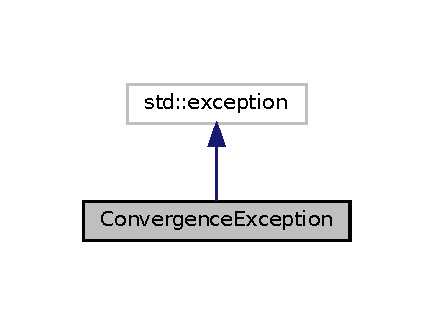
\includegraphics[width=208pt]{classConvergenceException__inherit__graph}
\end{center}
\end{figure}


Collaboration diagram for Convergence\+Exception\+:
\nopagebreak
\begin{figure}[H]
\begin{center}
\leavevmode
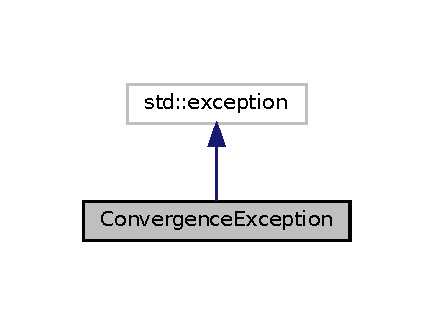
\includegraphics[width=208pt]{classConvergenceException__coll__graph}
\end{center}
\end{figure}
\subsection*{Public Member Functions}
\begin{DoxyCompactItemize}
\item 
\mbox{\Hypertarget{classConvergenceException_a316e0101d86b3df281451159d68bac38}\label{classConvergenceException_a316e0101d86b3df281451159d68bac38}} 
virtual const char $\ast$ {\bfseries what} () const  throw ()
\end{DoxyCompactItemize}


\subsection{Detailed Description}
Throw this when Xfoil calculation fails to converge. 

The documentation for this class was generated from the following files\+:\begin{DoxyCompactItemize}
\item 
/home/jesse/\+Git/\+Xfoil-\/\+Interface/headers/types.\+h\item 
/home/jesse/\+Git/\+Xfoil-\/\+Interface/src/types.\+cpp\end{DoxyCompactItemize}

\hypertarget{classpolar}{}\section{polar Class Reference}
\label{classpolar}\index{polar@{polar}}


Vector of vectors, for storing xfoil calculation results.  




{\ttfamily \#include $<$types.\+h$>$}



Inheritance diagram for polar\+:
\nopagebreak
\begin{figure}[H]
\begin{center}
\leavevmode
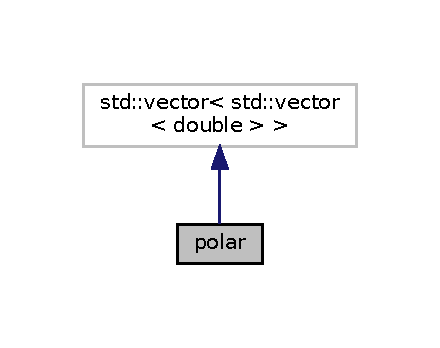
\includegraphics[width=211pt]{classpolar__inherit__graph}
\end{center}
\end{figure}


Collaboration diagram for polar\+:
\nopagebreak
\begin{figure}[H]
\begin{center}
\leavevmode
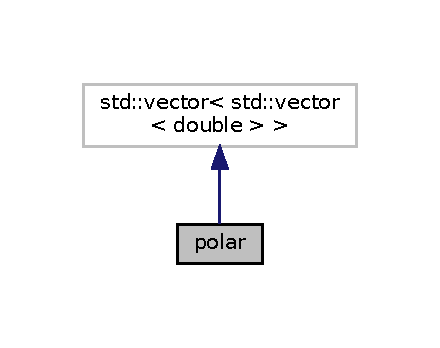
\includegraphics[width=211pt]{classpolar__coll__graph}
\end{center}
\end{figure}
\subsection*{Public Member Functions}
\begin{DoxyCompactItemize}
\item 
\mbox{\Hypertarget{classpolar_a98964526743174dcc56051b4e9ce4715}\label{classpolar_a98964526743174dcc56051b4e9ce4715}} 
{\bfseries polar} (size\+\_\+t lines)
\end{DoxyCompactItemize}
\subsection*{Public Attributes}
\begin{DoxyCompactItemize}
\item 
\mbox{\Hypertarget{classpolar_a1c55c9133a8862a41e91142d06c57a93}\label{classpolar_a1c55c9133a8862a41e91142d06c57a93}} 
std\+::vector$<$ std\+::vector$<$ double $>$ $>$ {\bfseries contents}
\end{DoxyCompactItemize}


\subsection{Detailed Description}
Vector of vectors, for storing xfoil calculation results. 

The documentation for this class was generated from the following files\+:\begin{DoxyCompactItemize}
\item 
/home/jesse/\+Git/\+Xfoil-\/\+Interface/headers/types.\+h\item 
/home/jesse/\+Git/\+Xfoil-\/\+Interface/src/types.\+cpp\end{DoxyCompactItemize}

\hypertarget{classXfoilInterface}{}\section{Xfoil\+Interface Class Reference}
\label{classXfoilInterface}\index{Xfoil\+Interface@{Xfoil\+Interface}}


Class that interfaces with X\+Foil.  




{\ttfamily \#include $<$xfoilinterface.\+h$>$}

\subsection*{Public Member Functions}
\begin{DoxyCompactItemize}
\item 
\mbox{\Hypertarget{classXfoilInterface_acf3d487c09b576a8730a23eb6decee57}\label{classXfoilInterface_acf3d487c09b576a8730a23eb6decee57}} 
\hyperlink{classXfoilInterface_acf3d487c09b576a8730a23eb6decee57}{Xfoil\+Interface} (bool plot, double Ncrit=9)
\begin{DoxyCompactList}\small\item\em Constructor for \hyperlink{classXfoilInterface}{Xfoil\+Interface} class. \end{DoxyCompactList}\item 
\mbox{\Hypertarget{classXfoilInterface_a48dc2121cd7710c73eee89643088ab7c}\label{classXfoilInterface_a48dc2121cd7710c73eee89643088ab7c}} 
\hyperlink{classXfoilInterface_a48dc2121cd7710c73eee89643088ab7c}{$\sim$\+Xfoil\+Interface} ()
\begin{DoxyCompactList}\small\item\em Destructor for \hyperlink{classXfoilInterface}{Xfoil\+Interface} class. \end{DoxyCompactList}\item 
bool \hyperlink{classXfoilInterface_aba502bd5accaf23d3bdf342a82d5fb7f}{start} ()
\begin{DoxyCompactList}\small\item\em Starts xfoil interface. \end{DoxyCompactList}\item 
\mbox{\Hypertarget{classXfoilInterface_aedc0b9716eb07c623b9577c69ad2cc97}\label{classXfoilInterface_aedc0b9716eb07c623b9577c69ad2cc97}} 
int \hyperlink{classXfoilInterface_aedc0b9716eb07c623b9577c69ad2cc97}{Configure} ()
\begin{DoxyCompactList}\small\item\em Configures xfoil with constructor parameters. \end{DoxyCompactList}\item 
\mbox{\Hypertarget{classXfoilInterface_a7225d1f5817cb79f9f938c8dc616a360}\label{classXfoilInterface_a7225d1f5817cb79f9f938c8dc616a360}} 
bool \hyperlink{classXfoilInterface_a7225d1f5817cb79f9f938c8dc616a360}{Quit} ()
\begin{DoxyCompactList}\small\item\em Quits xfoil. \end{DoxyCompactList}\item 
\mbox{\Hypertarget{classXfoilInterface_a21659717b7901562e97d25460e8c4f42}\label{classXfoilInterface_a21659717b7901562e97d25460e8c4f42}} 
bool \hyperlink{classXfoilInterface_a21659717b7901562e97d25460e8c4f42}{set\+Iter} (unsigned int iterations)
\begin{DoxyCompactList}\small\item\em sets number of iterations \end{DoxyCompactList}\item 
void \hyperlink{classXfoilInterface_ae6be41dc3be9e28cd36ed5e9a40b0854}{load\+Foil\+File} (char fpath\mbox{[}$\,$\mbox{]}, char foil_name\mbox{[}$\,$\mbox{]})
\begin{DoxyCompactList}\small\item\em Loads airfoil coordinates from file. \end{DoxyCompactList}\item 
void \hyperlink{classXfoilInterface_a202072a14053054a55501c45a296bce7}{N\+A\+CA} (const char code\mbox{[}5\mbox{]})
\begin{DoxyCompactList}\small\item\em Selects a N\+A\+CA airfoil to input_ to xfoil. \end{DoxyCompactList}\item
std\+::vector$<$ double $>$ \hyperlink{classXfoilInterface_a7937559afde3fe6880b64b4d8b278256}{angle\+Of\+Attack} (double angle)
\begin{DoxyCompactList}\small\item\em Starts Xfoil analysis of single angle of attack. \end{DoxyCompactList}\item 
\hyperlink{classpolar}{polar} \hyperlink{classXfoilInterface_ac2b547ba157afbb666ddf5f3eff271e2}{angle\+Of\+Attack} (double anglest, double anglee, double angleinc)
\begin{DoxyCompactList}\small\item\em Starts Xfoil analysis of sequence of angles. \end{DoxyCompactList}\item 
std\+::vector$<$ double $>$ \hyperlink{classXfoilInterface_a7dbc26399dc54c42d5e71d0d7cbb2d07}{lift\+Coefficient} (double liftcoeff)
\begin{DoxyCompactList}\small\item\em Starts Xfoil analysis of single lift coefficient. \end{DoxyCompactList}\item 
\hyperlink{classpolar}{polar} \hyperlink{classXfoilInterface_a04e40003487d76af5f29be2a26103fd3}{lift\+Coefficient} (double clstart, double clend, double clinc)
\begin{DoxyCompactList}\small\item\em Starts Xfoil analysis of sequence of lift coefficients. \end{DoxyCompactList}\item 
\mbox{\Hypertarget{classXfoilInterface_a80e8724704363aa11365f79b338bf20c}\label{classXfoilInterface_a80e8724704363aa11365f79b338bf20c}} 
bool \hyperlink{classXfoilInterface_a80e8724704363aa11365f79b338bf20c}{set\+Viscosity} (unsigned int Reynolds)
\begin{DoxyCompactList}\small\item\em Enables viscous mode. \end{DoxyCompactList}\end{DoxyCompactItemize}


\subsection{Detailed Description}
Class that interfaces with X\+Foil. 

\subsection{Member Function Documentation}
\mbox{\Hypertarget{classXfoilInterface_a7937559afde3fe6880b64b4d8b278256}\label{classXfoilInterface_a7937559afde3fe6880b64b4d8b278256}} 
\index{Xfoil\+Interface@{Xfoil\+Interface}!angle\+Of\+Attack@{angle\+Of\+Attack}}
\index{angle\+Of\+Attack@{angle\+Of\+Attack}!Xfoil\+Interface@{Xfoil\+Interface}}
\subsubsection{\texorpdfstring{angle\+Of\+Attack()}{AngleOfAttack()}\hspace{0.1cm}{\footnotesize\ttfamily [1/2]}}
{\footnotesize\ttfamily std\+::vector$<$ double $>$ Xfoil\+Interface\+::angle\+Of\+Attack (\begin{DoxyParamCaption}\item[{double}]{angle }\end{DoxyParamCaption})}



Starts Xfoil analysis of single angle of attack. 


\begin{DoxyParams}{Parameters}
{\em angle} & angle of attack to analyze \\
\hline
\end{DoxyParams}
\begin{DoxyReturn}{Returns}
vector containing calculation results, same order as input_ xfoil polar files
\end{DoxyReturn}
\mbox{\Hypertarget{classXfoilInterface_ac2b547ba157afbb666ddf5f3eff271e2}\label{classXfoilInterface_ac2b547ba157afbb666ddf5f3eff271e2}} 
\index{Xfoil\+Interface@{Xfoil\+Interface}!angle\+Of\+Attack@{angle\+Of\+Attack}}
\index{angle\+Of\+Attack@{angle\+Of\+Attack}!Xfoil\+Interface@{Xfoil\+Interface}}
\subsubsection{\texorpdfstring{angle\+Of\+Attack()}{AngleOfAttack()}\hspace{0.1cm}{\footnotesize\ttfamily [2/2]}}
{\footnotesize\ttfamily \hyperlink{classpolar}{polar} Xfoil\+Interface\+::angle\+Of\+Attack (\begin{DoxyParamCaption}\item[{double}]{anglest,  }\item[{double}]{anglee,  }\item[{double}]{angleinc }\end{DoxyParamCaption})}



Starts Xfoil analysis of sequence of angles. 


\begin{DoxyParams}{Parameters}
{\em anglest} & starting angle of sequence \\
\hline
{\em anglee} & ending angle of sequence \\
\hline
{\em angleinc} & angle increment \\
\hline
{\em liftcoeffs} & array to store results input_ \\
\hline
\end{DoxyParams}
\begin{DoxyReturn}{Returns}
polar file data structure 
\end{DoxyReturn}
\mbox{\Hypertarget{classXfoilInterface_a7dbc26399dc54c42d5e71d0d7cbb2d07}\label{classXfoilInterface_a7dbc26399dc54c42d5e71d0d7cbb2d07}} 
\index{Xfoil\+Interface@{Xfoil\+Interface}!lift\+Coefficient@{lift\+Coefficient}}
\index{lift\+Coefficient@{lift\+Coefficient}!Xfoil\+Interface@{Xfoil\+Interface}}
\subsubsection{\texorpdfstring{lift\+Coefficient()}{LiftCoefficient()}\hspace{0.1cm}{\footnotesize\ttfamily [1/2]}}
{\footnotesize\ttfamily std\+::vector$<$ double $>$ Xfoil\+Interface\+::lift\+Coefficient (\begin{DoxyParamCaption}\item[{double}]{liftcoeff }\end{DoxyParamCaption})}



Starts Xfoil analysis of single lift coefficient. 


\begin{DoxyParams}{Parameters}
{\em liftcoeff} & Lift coefficient to analyze \\
\hline
\end{DoxyParams}
\begin{DoxyReturn}{Returns}
vector containing calculation results, same order as input_ xfoil polar files
\end{DoxyReturn}
\mbox{\Hypertarget{classXfoilInterface_a04e40003487d76af5f29be2a26103fd3}\label{classXfoilInterface_a04e40003487d76af5f29be2a26103fd3}} 
\index{Xfoil\+Interface@{Xfoil\+Interface}!lift\+Coefficient@{lift\+Coefficient}}
\index{lift\+Coefficient@{lift\+Coefficient}!Xfoil\+Interface@{Xfoil\+Interface}}
\subsubsection{\texorpdfstring{lift\+Coefficient()}{LiftCoefficient()}\hspace{0.1cm}{\footnotesize\ttfamily [2/2]}}
{\footnotesize\ttfamily \hyperlink{classpolar}{polar} Xfoil\+Interface\+::lift\+Coefficient (\begin{DoxyParamCaption}\item[{double}]{clstart,  }\item[{double}]{clend,  }\item[{double}]{clinc }\end{DoxyParamCaption})}



Starts Xfoil analysis of sequence of lift coefficients. 


\begin{DoxyParams}{Parameters}
{\em clstart} & starting lift coefficient \\
\hline
{\em clend} & ending lift coefficient \\
\hline
{\em clinc} & lift coefficient increment \\
\hline
{\em angles} & array to store results input_ \\
\hline
\end{DoxyParams}
\begin{DoxyReturn}{Returns}
Polar file data structure 
\end{DoxyReturn}
\mbox{\Hypertarget{classXfoilInterface_ae6be41dc3be9e28cd36ed5e9a40b0854}\label{classXfoilInterface_ae6be41dc3be9e28cd36ed5e9a40b0854}} 
\index{Xfoil\+Interface@{Xfoil\+Interface}!load\+Foil\+File@{load\+Foil\+File}}
\index{load\+Foil\+File@{load\+Foil\+File}!Xfoil\+Interface@{Xfoil\+Interface}}
\subsubsection{\texorpdfstring{load\+Foil\+File()}{LoadFoilFile()}}
{\footnotesize\ttfamily void Xfoil\+Interface\+::load\+Foil\+File (\begin{DoxyParamCaption}\item[{char}]{fpath\mbox{[}$\,$\mbox{]},  }\item[{char}]{foil_name\mbox{[}$\,$\mbox{]} }\end{DoxyParamCaption})}



Loads airfoil coordinates from file. 


\begin{DoxyParams}{Parameters}
{\em fpath} & File to load coordinates from \\
\hline
{\em foil_name} & Airfoil name \\
\hline
\end{DoxyParams}
\mbox{\Hypertarget{classXfoilInterface_a202072a14053054a55501c45a296bce7}\label{classXfoilInterface_a202072a14053054a55501c45a296bce7}} 
\index{Xfoil\+Interface@{Xfoil\+Interface}!N\+A\+CA@{N\+A\+CA}}
\index{N\+A\+CA@{N\+A\+CA}!Xfoil\+Interface@{Xfoil\+Interface}}
\subsubsection{\texorpdfstring{N\+A\+C\+A()}{NACA()}}
{\footnotesize\ttfamily void Xfoil\+Interface\+::\+N\+A\+CA (\begin{DoxyParamCaption}\item[{const char}]{code\mbox{[}5\mbox{]} }\end{DoxyParamCaption})}



Selects a N\+A\+CA airfoil to input_ to xfoil.


\begin{DoxyParams}{Parameters}
{\em input_} & 4-\/digit naca airfoil code \\
\hline
\end{DoxyParams}
\mbox{\Hypertarget{classXfoilInterface_aba502bd5accaf23d3bdf342a82d5fb7f}\label{classXfoilInterface_aba502bd5accaf23d3bdf342a82d5fb7f}} 
\index{Xfoil\+Interface@{Xfoil\+Interface}!start@{start}}
\index{start@{start}!Xfoil\+Interface@{Xfoil\+Interface}}
\subsubsection{\texorpdfstring{start()}{Start()}}
{\footnotesize\ttfamily bool Xfoil\+Interface\+::start (\begin{DoxyParamCaption}{ }\end{DoxyParamCaption})}



Starts xfoil interface. 

\begin{DoxyReturn}{Returns}
Whether X\+Foil was initialized succesfully 
\end{DoxyReturn}


The documentation for this class was generated from the following files\+:\begin{DoxyCompactItemize}
\item 
/home/jesse/\+Git/\+Xfoil-\/\+Interface/headers/\hyperlink{xfoilinterface_8h}{xfoilinterface.\+h}\item 
/home/jesse/\+Git/\+Xfoil-\/\+Interface/src/xfoilinterface.\+cpp\end{DoxyCompactItemize}

\chapter{File Documentation}
\hypertarget{xfoilinterface_8h}{}\section{/home/jesse/\+Git/\+Xfoil-\/\+Interface/headers/xfoilinterface.h File Reference}
\label{xfoilinterface_8h}\index{/home/jesse/\+Git/\+Xfoil-\/\+Interface/headers/xfoilinterface.\+h@{/home/jesse/\+Git/\+Xfoil-\/\+Interface/headers/xfoilinterface.\+h}}


Library for calling X\+Foil from a C++ program.  


{\ttfamily \#include \char`\"{}include.\+h\char`\"{}}\newline
{\ttfamily \#include \char`\"{}types.\+h\char`\"{}}\Newline
Include dependency graph for xfoilinterface.\+h\+:
\nopagebreak
\begin{figure}[H]
\begin{center}
\leavevmode
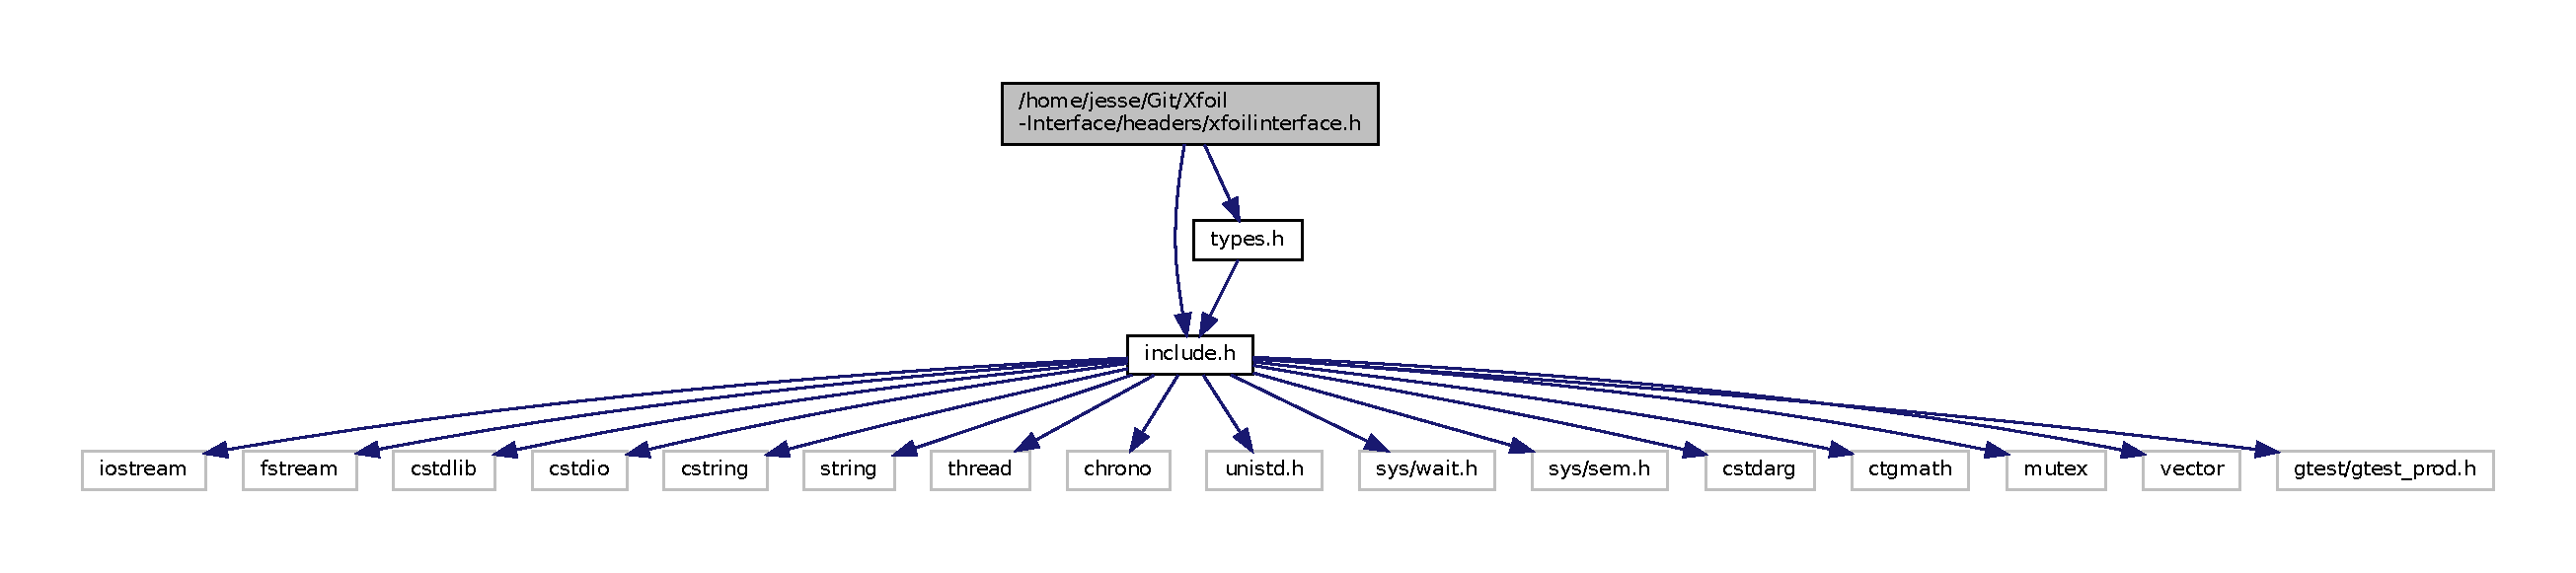
\includegraphics[width=350pt]{xfoilinterface_8h__incl}
\end{center}
\end{figure}
\subsection*{Classes}
\begin{DoxyCompactItemize}
\item 
class \hyperlink{classXfoilInterface}{Xfoil\+Interface}
\begin{DoxyCompactList}\small\item\em Class that interfaces with X\+Foil. \end{DoxyCompactList}\end{DoxyCompactItemize}
\subsection*{Macros}
\begin{DoxyCompactItemize}
\item 
\mbox{\Hypertarget{xfoilinterface_8h_aa356ef02781a247c145c64579cd59cd1}\label{xfoilinterface_8h_aa356ef02781a247c145c64579cd59cd1}} 
\#define {\bfseries P\+A\+C\+C\+\_\+\+F\+A\+IL}~(-\/1)
\item 
\mbox{\Hypertarget{xfoilinterface_8h_a93681b5eaf558e5fa9434775dfae6de5}\label{xfoilinterface_8h_a93681b5eaf558e5fa9434775dfae6de5}} 
\#define {\bfseries V\+I\+S\+C\+\_\+\+F\+A\+IL}~(-\/2)
\item 
\mbox{\Hypertarget{xfoilinterface_8h_a1dc91fc1ff605b8dbf72bff317ab2228}\label{xfoilinterface_8h_a1dc91fc1ff605b8dbf72bff317ab2228}} 
\#define {\bfseries I\+T\+E\+R\+\_\+\+F\+A\+IL}~(-\/3)
\item 
\mbox{\Hypertarget{xfoilinterface_8h_a06ca5895c2ac8b63a56eba16f35230cc}\label{xfoilinterface_8h_a06ca5895c2ac8b63a56eba16f35230cc}} 
\#define {\bfseries I\+N\+P\+U\+T\+\_\+\+L\+OG}
\item 
\mbox{\Hypertarget{xfoilinterface_8h_a8e3a929ca84c198906db175852672ab6}\label{xfoilinterface_8h_a8e3a929ca84c198906db175852672ab6}} 
\#define {\bfseries C\+M\+D\+\_\+\+B\+U\+F\+F\+\_\+\+S\+I\+ZE}~1024
\item 
\mbox{\Hypertarget{xfoilinterface_8h_a7dcea8d404f7a8401945947546880002}\label{xfoilinterface_8h_a7dcea8d404f7a8401945947546880002}} 
\#define {\bfseries O\+U\+T\+P\+U\+T\+\_\+\+B\+U\+F\+F\+\_\+\+S\+I\+ZE}~200
\item 
\mbox{\Hypertarget{xfoilinterface_8h_a568e4550c80c1defe0e2a759d1f84cdc}\label{xfoilinterface_8h_a568e4550c80c1defe0e2a759d1f84cdc}} 
\#define {\bfseries S\+E\+T\+T\+I\+N\+G\+S\+\_\+\+P\+R\+O\+C\+E\+S\+S\+\_\+\+T\+I\+ME}~10
\item 
\mbox{\Hypertarget{xfoilinterface_8h_a06a706d3b8c162066ad5f1f0b2183827}\label{xfoilinterface_8h_a06a706d3b8c162066ad5f1f0b2183827}} 
\#define {\bfseries P\+O\+L\+A\+R\+\_\+\+D\+A\+T\+A\+\_\+\+L\+I\+N\+E\+NR}~12
\item 
\mbox{\Hypertarget{xfoilinterface_8h_aa8c9032162923f4f0ed32b1561405c92}\label{xfoilinterface_8h_aa8c9032162923f4f0ed32b1561405c92}} 
\#define {\bfseries Parent\+Read}~inpipe_\mbox{[}0\mbox{]}
\item 
\mbox{\Hypertarget{xfoilinterface_8h_ad368fe448ed30e0cb157c01aa8455a4c}\label{xfoilinterface_8h_ad368fe448ed30e0cb157c01aa8455a4c}} 
\#define {\bfseries Parent\+Write}~outpipe_\mbox{[}1\mbox{]}
\item 
\mbox{\Hypertarget{xfoilinterface_8h_a24175bbb0972e1e53b5af29abee03e17}\label{xfoilinterface_8h_a24175bbb0972e1e53b5af29abee03e17}} 
\#define {\bfseries Child\+Read}~outpipe_\mbox{[}0\mbox{]}
\item 
\mbox{\Hypertarget{xfoilinterface_8h_a724188c0cc2d080a0ac5f3a01bf6cb47}\label{xfoilinterface_8h_a724188c0cc2d080a0ac5f3a01bf6cb47}} 
\#define {\bfseries Child\+Write}~inpipe_\mbox{[}1\mbox{]}
\end{DoxyCompactItemize}


\subsection{Detailed Description}
Library for calling X\+Foil from a C++ program. 

\begin{DoxyAuthor}{Author}
Jesse van Rhijn 
\end{DoxyAuthor}

%--- End generated contents ---

% Index
\backmatter
\newpage
\phantomsection
\clearemptydoublepage
\addcontentsline{toc}{chapter}{Index}
\printindex

\end{document}
